% Wilson loop linking number — illustrates Lk(K,L) for the expectation value
% <W_K W_L> ~ exp(2*pi*i * (k/4*pi) * Lk(K,L)) in U(1) Chern-Simons theory.
% Loop K bounds the shaded Seifert surface S_K; loop L pierces S_K once.
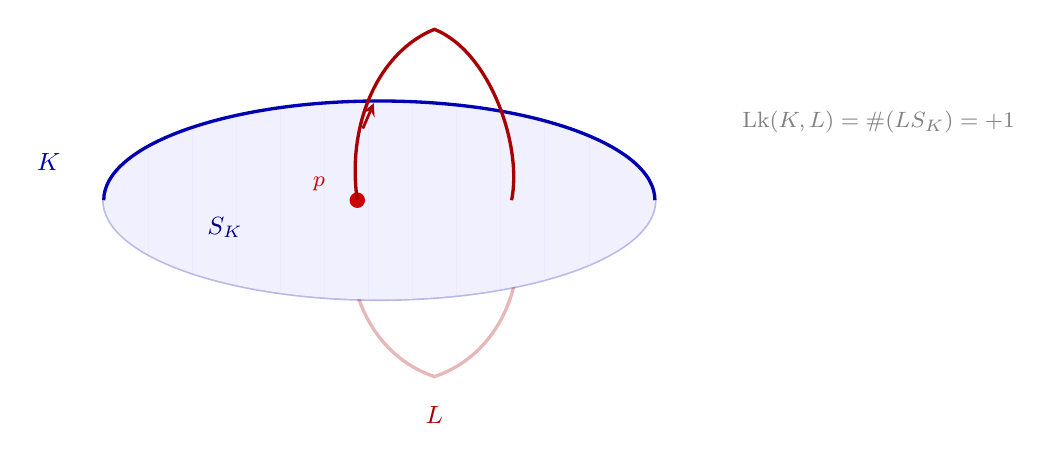
\begin{tikzpicture}[scale=1.4, thick,
    loop K/.style={very thick, blue!70!black},
    loop L/.style={very thick, red!65!black},
    surface/.style={fill=blue!6},
    faded/.style={opacity=0.28}]

  % Geometry:
  %   K = horizontal ellipse at y=0 (boundary of S_K), radii 2.5 x 0.9
  %   L = vertical ellipse centered at (0.5, 0), radii 0.9 x 1.7
  %       L passes through S_K at one point
  %
  % Drawing order (back to front):
  %   1. Back arc of K
  %   2. Back arc of L (below surface)
  %   3. Surface fill S_K
  %   4. Front arc of K
  %   5. Intersection point
  %   6. Front arc of L (above surface, with crossing over K)

  % === 1. Back arc of K ===
  \draw[loop K, faded] (180:2.5 and 0.9) arc (180:360:2.5 and 0.9);

  % === 2. Back arc of L (below the surface plane) ===
  % Parameterize L as an ellipse: center (0.5, 0), going from bottom up on left,
  % down on right. The "back" is the lower half.
  \draw[loop L, faded]
    (-0.2, 0.0)
    .. controls (-0.4, -0.7) and (-0.1, -1.4) .. (0.5, -1.6)
    .. controls (1.1, -1.4) and (1.4, -0.7) .. (1.2, 0.0);

  % === 3. Seifert surface S_K (fills over back arcs) ===
  \fill[surface] (0,0) ellipse (2.5 and 0.9);
  % Subtle vertical hatching
  \foreach \x in {-2.1,-1.7,...,2.1} {
    \pgfmathsetmacro{\ymax}{0.9*sqrt(max(0.001, 1 - (\x/2.5)*(\x/2.5)))}
    \draw[blue!8, very thin] (\x, -\ymax) -- (\x, \ymax);
  }

  % === 4. Front arc of K ===
  \draw[loop K] (180:2.5 and 0.9) arc (180:0:2.5 and 0.9);

  % === 5. Intersection point p (L emerges here) ===
  \fill[red!80!black] (-0.2, 0.0) circle (2pt);

  % === 6. Front arc of L (above the surface) ===
  % Drawn after K → naturally renders on top (over-crossing convention).
  \draw[loop L]
    (-0.2, 0.0)
    .. controls (-0.3, 0.7) and (0.0, 1.35) .. (0.5, 1.55)
    .. controls (1.0, 1.35) and (1.3, 0.5) .. (1.2, 0.0);

  % === Orientation arrow on L (ascending side, away from crossings) ===
  \draw[red!65!black, ->, >=stealth, line width=1pt]
    (-0.15, 0.65) -- (-0.05, 0.88);

  % === Labels ===
  \node[blue!70!black, font=\small, anchor=east] at (-2.8, 0.35) {$K$};
  \node[red!65!black, font=\small] at (0.5, -1.95) {$L$};
  \node[blue!50!black, font=\small] at (-1.4, -0.25) {$S_K$};
  \node[red!80!black, font=\footnotesize, anchor=east] at (-0.4, 0.15) {$p$};

  % === Annotation ===
  \node[font=\footnotesize, gray, anchor=north west] at (3.2, 0.9)
    {$\mathrm{Lk}(K,L) = \#(L \pitchfork S_K) = +1$};

\end{tikzpicture}
